\chapter{TonePrint Community concept}
\label{CommunityConcept}
In order to accommodate the research question of how methods of user centered design may be applied for the design process of the TonePrint community, it's desired to establish a model of the TonePrint community based on the knowledge obtained through the thematic analysis of the interview in \autoref{ThemanticAnalysis}. This model will serve as a base when deciding the tasks that lies ahead, in which user centered design methods may be applied.

\section{Conceptual model}
\label{ConceptualModel}
In \parencite[17]{PDF:Henderson2012} a conceptual model is descried  as "\textit{A high-level description of an application. It enumerates all concepts in the application that users can encounter, describes how those concepts relate to each other, and explains how those concepts fit into tasks that users perform with the application}".\\
In order to compose a conceptual model of the TonePrint community it's necessary to decide which features and functionalities that needs to be implemented and how they interact with one another. Since these decisions haven't yet been taken on a business level, does the decisions presented in this section only serve the purpose of this project. The decisions is based on interview with the development team of the TonePrint app.

\subsection{The TonePrint Concept model}
\label{TonePrintConceptualModel}
When creating the conceptual model it's necessary to look at the task domains in which the user till perform activities to reach their goal. Different users have different purposes for using the community and therefore will there be more than one task domain to consider, while designing the community. For this suitable to look at the different target user groups, which shortly is mentioned in \autoref{ThematicFindings}.\\
On \autoref{fig:TonePrintUserConpt} it's depicted how users of the TonePrint concept are categorized into the three groups, Pedal only users, TonePrint Users and TonePrint creators, And what aspects of the TonePrint concept they uses. The 'Pedal only users' are defined as the users who own a TonePrint pedal, but doesn't use the TonePrint functionalities of the pedal and just are using it as a regular pedal. The TonePrint Users are defined as those who use the TonePrint concept to find and beam Artist TonePrints to their pedals. These users are therefore connected to the Artist Library of the TonePrint application. The TonePrint Creators are defined as those who uses the TonePrint concept to create User TonePrints, which they can use with their pedals. These users are therefore connected to the Editor and the User TonePrint Library. The connecting arrow between TonePrint Users and Creators on \autoref{fig:TonePrintUserConpt} indicates that these users isn't necessary different people, but might be the same user using the system differently. 

\begin{figure}[H]
	\centering
	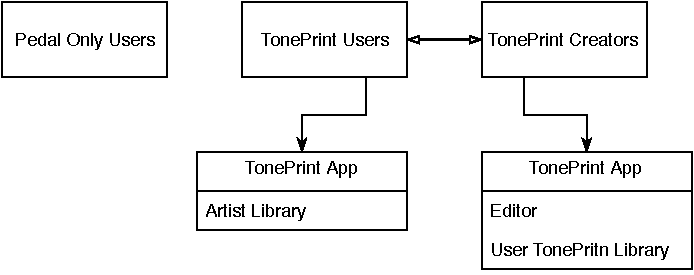
\includegraphics[width=0.85\textwidth]{TonePrintConcept.pdf}
	\caption{This illustrates the different groups of users of the TonePrint concept}
	\label{fig:TonePrintUserConpt}
\end{figure}

The definition of the different user groups of the TonePrint concept will also be applied to the concept of the TonePrint Community, besides the 'Pedal Only Users'. This is because they aren't using the TonePrint functions and thereby don't have any use of the TonePrint Community. The features listed in \autoref{tab:ListOfCommunityFeatures} are suggested features to accommodate both the TonePrint users and creators in the community. The features are based on the ideas and suggestions from the development team through the interview.

\begin{table}[H]
	\centering
\begin{tabular}[width=\textwidth]{c|l}
\textbf{Ref. nr} & \textbf{Features} \\ \hline
1 & Uploading TonePrints \\ \hline
2 & Categorize by tags \\ \hline
3 & TonePrint description \\ \hline
4 & Search \\ \hline
5 & Rate TonePrint \\ \hline
6 & Subscribe to users \\ \hline
7 & Recommendations \\ \hline
8 & User profile \\ \hline
\end{tabular}
\caption{The left column contains the number which is used to refer to the feature in the right column}
\label{tab:ListOfCommunityFeatures}
\end{table}

The features 1, 2 and 3 in \autoref{tab:ListOfCommunityFeatures} are all closely related and accommodates especially the task domain of the TonePrint Creators. The feature of uploading is simply to enable user to upload TonePrints to the community, that they have created with the editor. This feature covers the main function requested by the users which is the ability to share TonePrint with each other. \\
Feature 2, Categorizing by tags refers to the idea of letting users use tags to categorize the TonePrint they have uploaded. The purpose of these tags are to easily allow other users to identify which categories the TonePrint belongs to, which also enable users to find the TonePrints by searching on desired tags.\\
Feature 3, TonePrint description allows the creator of a TonePrint to write about the TonePrint, similar to the descriptions of the Artist TonePrints in the current TonePrint application. The description might contain information about the parameter settings, inspiration, self-promoting text or likewise. \\
Feature 4 is a search function which users can use to search for TonePrints, either by name, tag, artist, pedal or likewise. The current search functionality in the TonePrint application, which only is idle for android, is very limited and wouldn't be sufficient, as mentioned in \autoref{AppendixHeuristics}. \\
Feature 5, the Rate TonePrint feature, is based on the idea of letting TonePrint users, who have tried a TonePrint creators TonePrint, rate that TonePrint. This rating could work as a motivation for creators to create more TonePrints, while it as the same time gives the TonePrint users the opportunity to see how much other users like the TonePrint. \\
Feature 6, Subscribe to users, are a feature which enables users to follow other users. A user could for instance have tried a TonePrint created by a certain other user and like it to a degree of which he want's to see which other TonePrints that user have created, and wants to be notified when new ones are created.\\
Feature 7, Recommendation, this feature is suggested to help users find and explore TonePrints. This could be recommendations like, "People who like this TonePrint also like these", "These are the highest rated TonePrints for your pedals" or "These TonePrints will at something new" etc.\\
Feature 8, Community Profile, is a feature which sums it all up. This profile is going to be a 'Front Page' for the users containing their own TonePrints, their recommendations, the TonePrints of those they subscribe to and the option to make a personal description and link to personal youtube, soundcloud or likewise sites, as a self-promoting feature.\\
\\
How the eight features above works on a detailed and technical level won't be a concern at the conceptual model. The goal of the conceptual model is to explain the relationship between functions, which can be used to perform the activities necessary for the user to reach a goal \parencite{Henderson2012}.


\subsection{Community Model}
\label{CommunityModel}
The conceptual model of the TonePrint community consists of several concepts, which includes the already mentioned features \autoref{tab:ListOfCommunityFeatures}. The conceptual model of the TonePrint community is illustrated on \autoref{fig:CommunityConceptualModel}.\\

\begin{figure}[H]
	\centering
	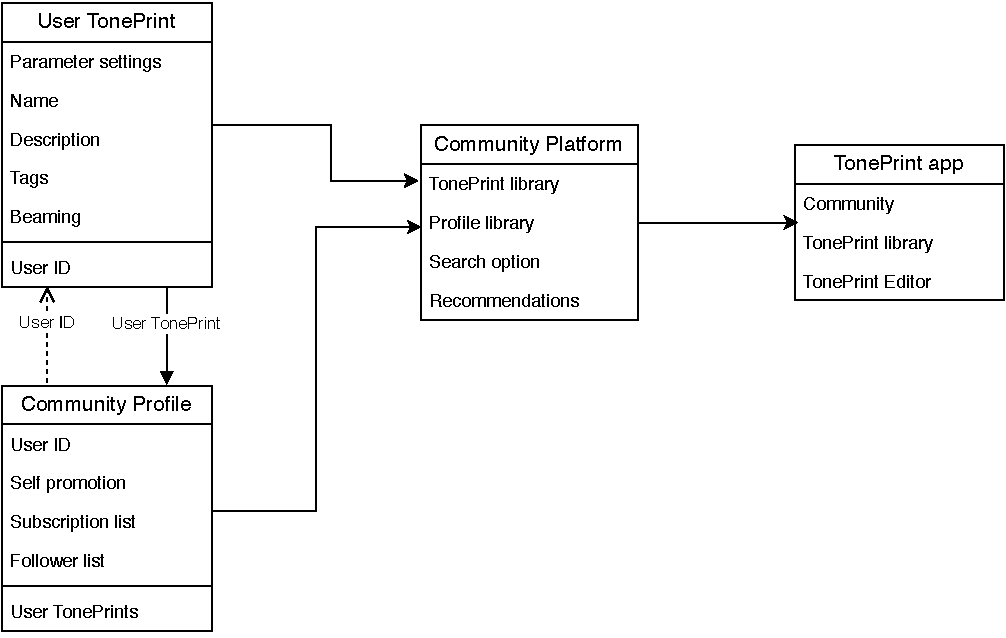
\includegraphics[width=0.90\textwidth]{CommunityNewDraft.pdf}
	\caption{Illustration of the relationships of the concepts that makes up the Communities conceptual model}
	\label{fig:CommunityConceptualModel}
\end{figure}

The first concept in the model is the User TonePrint concept, which contains the following: Parameter settings for the TonePrint. The name of the TonePrint. A description of the TonePrint. Tags that categorize the TonePrint . The beaming functionality. And lastly User ID, which is inherited from the Community Profile, which identifies the creator. This concepts differs from the original User TonePrint concept by adding the description, tags and User ID, which all are new additions, which aims at making it easier to find desired TonePrints. The User TonePrints are uploaded to the Communitys TonePrint library, for all user to find. It's also uploaded to the users own Community Profile so it's always easy accessible.\\
The second concept of the model is the Community Profile which contains: User ID that is used to identify the profile. Self-promotion which could include self description or links to other personal sites etc. Subscription list, which is a list of the other user that a user are subscribing to. Follower list, which is a list of those who subscribe to that user. And lastly the User TonePrints which is a list of the users self created TonePrints. The Community Profile is crucial to shape the concept of including the users into a community, instead of just having a simple Upload/Download site. Some of the idea of self-promotion stems from a workshop conducted by TC \parencite{PDF:BrugerWorkshopUserTonePrints}. The Community profile will work as a starting point for users when interacting with the Community.\\
The third concept is the Community platform which contains: The TonePrint library which give access to use and rate all the uploaded TonePrints. The Profile library give access to visit all of the Community Profiles and subscribe to them. Search option is simply a function which help user find the TonePrint they are looking fore, e.g by searching on the before mentioned tags. Recommendations where the system suggest TonePrints or users based on the TonePrints they use or likes. The Community Platform sums up all of the features and concepts which shapes the TonePrint community concept, by using both the User TonePrint concept and the Community Profile concept.\\
Lastly there is the concept of the TonePrint application which contains: The Community Platform, which represent all of the features and concepts of the TonePrint Community. The TonePrint library represent both the User TonePrint library and the Artist TonePrint library, first described in \autoref{TonePrintSoftware}, and seen in \autoref{fig:TonePrintUserConpt}. The TonePrint Editor, which is used to create the User TonePrints, which is described in \autoref{TonePrintSoftware} and seen in \autoref{fig:TonePrintUserConpt}. The only change in the TonePrint application concept is the addition of the Community concept. As mentioned in \autoref{ThematicFindings} is there still some different viewpoints regarding the extend of the TonePrint concept being a part of the current TonePrint app. 

\subsection{Community Use Cases}
\label{CommunityUseCases}
Contrary to the Conceptual model that depicts how the different concepts of the tonePrint Community are connected, is the scope of the use cases to depict how the TonePrint Community is used to complete the tasks that users might use it fore. The use cases depict in this section is used to illustrate the overall idea of the use of the TonePrint community. The use cases is used provide a broader idea of the TonePrint community concept.\\
The two use cases described below is created to accommodate the use of the two user groups depicted in \autoref{fig:TonePrintUserConpt}.

\subsubsection*{TonePrint creator}
\label{UseCase1}
%
A use case of the TonePrint community for the user grouped earlier defined as TonePrint creators is to create and upload a TonePrint, so that it may be used by other users. This use case is illustrated on \autoref{fig:CommunityUseCase}. The four boxes in \autoref{fig:CommunityUseCase} represent Two users (User 1 and User 2) and two platforms of the tonePrint app (TonePrint Editor and Community Platform). User 1 represents a TonePrint creator. At the beginning of this use case User 1 uses the TonePrint editor to set the parameters of the TonePrint being created, which after it's given a name and is saved. User 1 hereafter uploads the TonePrint to the community platform. As a part of the uploading process User 1 write a description of the TonePrint, so that other users may want to try it out. User 1 also assigns tags to the TonePrint that may help categorize it, and make it show up when other users searches for one of the tags. 

\subsection*{TonePrint user}
\label{UseCase2}
%
The use case for the user group earlier defined as TonePrint users is also illustrated in \autoref{fig:CommunityUseCase}. Here it's seen that user 2 interacts with the Community Platform in order to find a TonePrint to use. User 2 searches for a TonePrint, which could be done by searching for specific pedals, effect types, other users (TonePrint creators) or tags that categorize the TonePrint. After finding a TonePrint, which in this case is created by User 1, is User 2 trying out the TonePrint by playing by beaming it to his pedal and playing on his guitar. After User 2 have decided that he likes it he rate it, so that other user might see that it's a good TonePrint. Finally User 2 chooses to subscribe to User 1 so that he will be notified when User 1 creates a new TonePrint.


\begin{figure}[H]
	\centering
	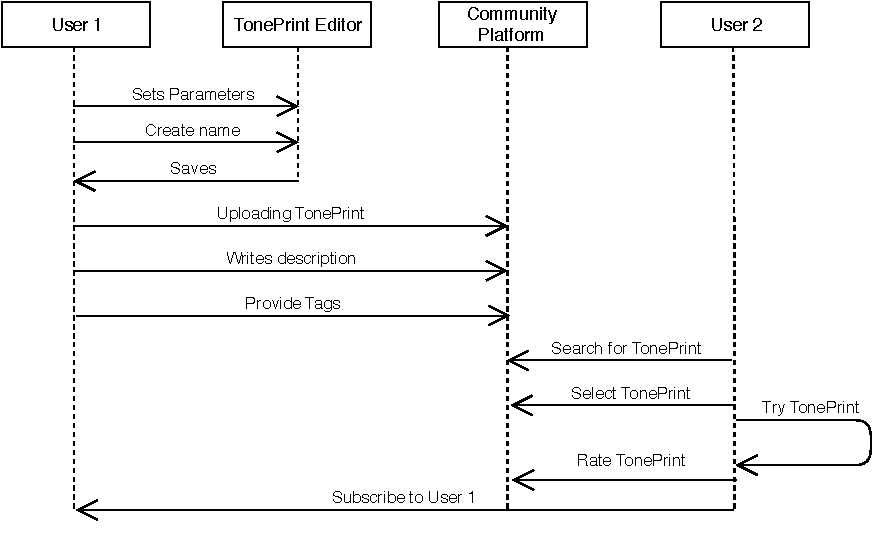
\includegraphics[width=0.95\textwidth]{UseCases.pdf}
	\caption{a graphical overview of the TonePrint Community use case}
	\label{fig:CommunityUseCase}
\end{figure}